\documentclass[]{scrartcl}
\usepackage{graphicx}
\usepackage{hyperref}
\hypersetup{
    colorlinks=true,
    linkcolor=blue,
    filecolor=magenta,      
    urlcolor=cyan,
}
\urlstyle{same}

\begin{document}

\title{Jupyterhub \\ \url{https://fhnw.netlabs.ch}}
\maketitle

\section{\"Ubersicht}

Die \href{https://jupyter.org/hub}{Jupyterhub}-Installation auf \url{https://fhnw.netlabs.ch/} bietet einfachen Zugriff auf \href{}{Jupyter-Notebooks} und ``Terminal''-Sessions (shell).

Es macht einfach mehr Spass selber mit den (Terminal) Tools rumzuspielen als
nur zuzuschauen (vergleiche \"Ubungs-Slides in den Folien).

\section{Verwenden des Terminals/`shell`}

\subsection*{Jupyter-Server starten}
Nach einloggen in das Portal muss zuerst ein ``eigener'' Jupyter-Server gestartet werden -- das ist ein Python-Prozess mit \texttt{ipython}/\texttt{juypiternotebook}:

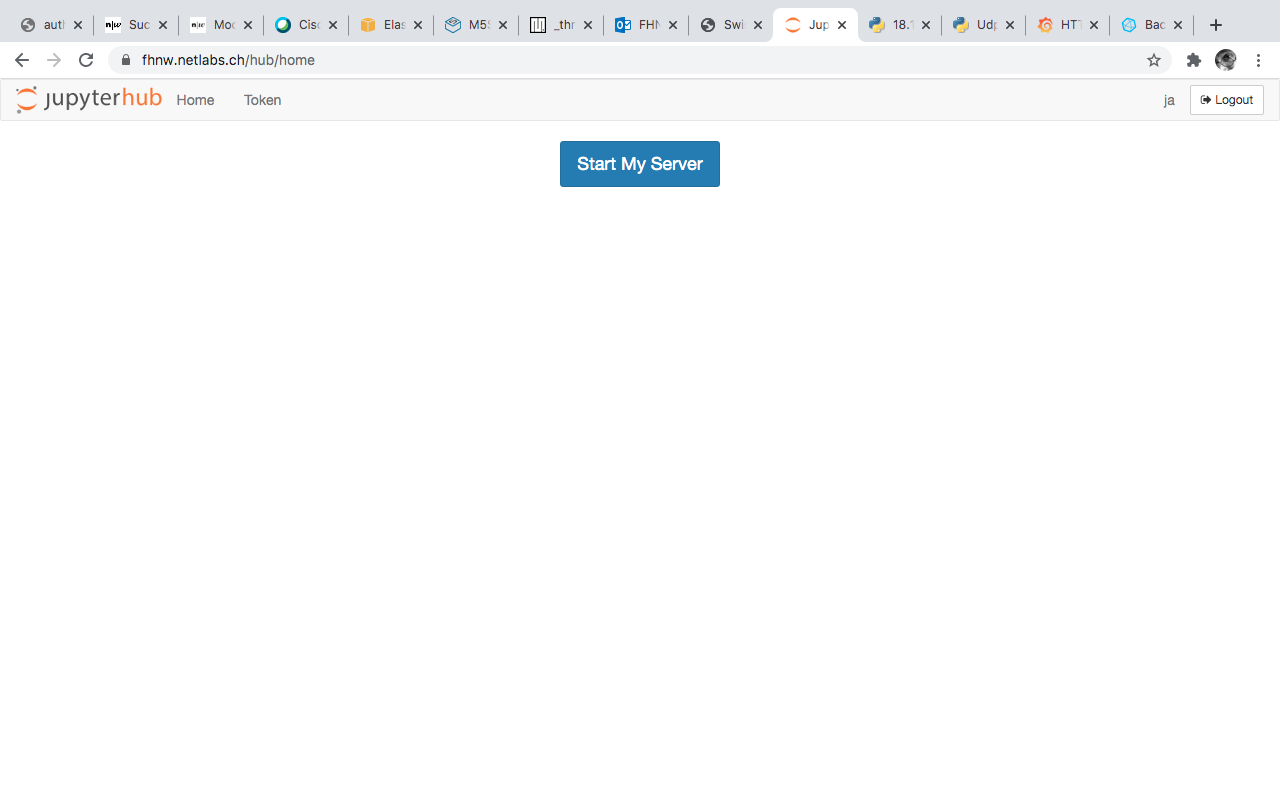
\includegraphics[width=10cm]{jupyterhub/jupyterhub_start_server}

\subsection*{Terminal starten}
Sie befinden sich nun in Ihrem pers\"onlichen Jupyter-Notebook und k\"onnen
\"uber ``New'' ein neues Notebook oder eben Terminal instanzieren (ein neues Fenster/Tab wird ge\"offnet):

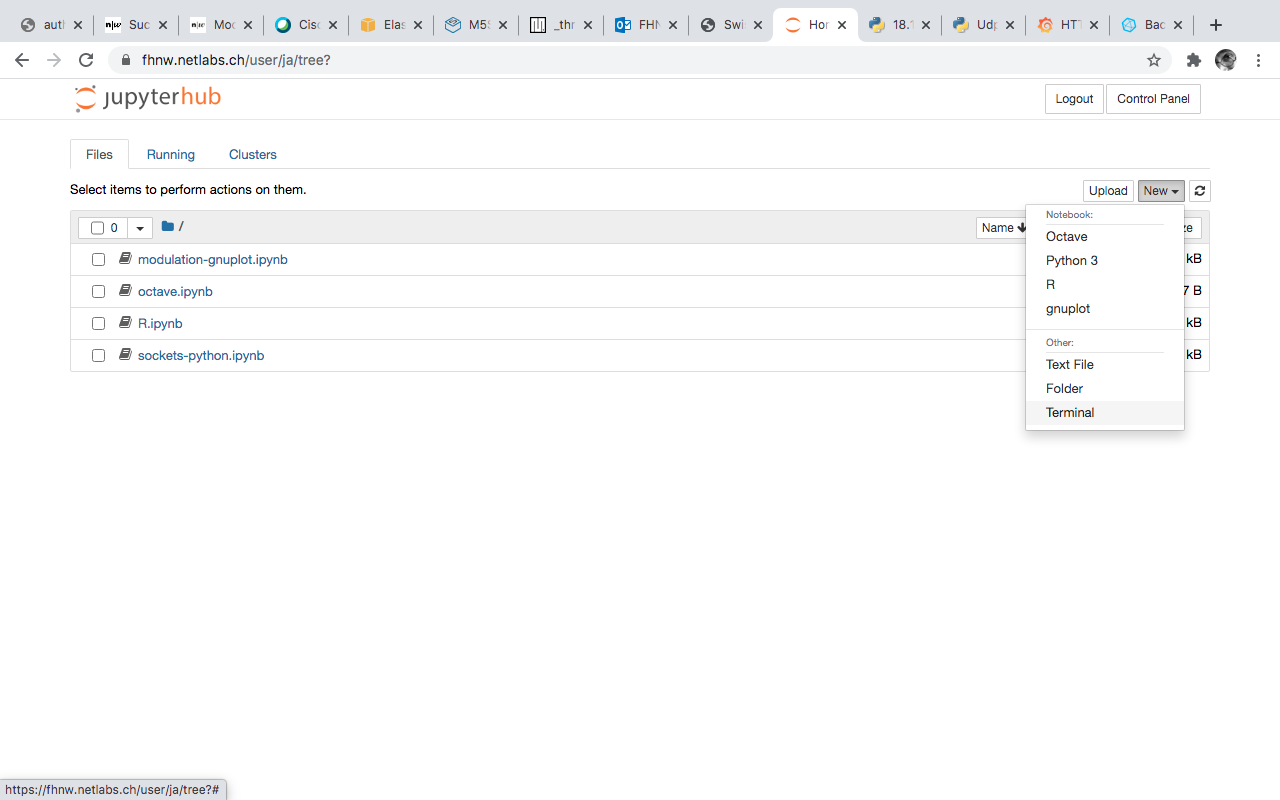
\includegraphics[width=10cm]{jupyterhub/jupyterhub_start_terminal}

\subsection*{Terminal benutzen}
Die in den Folien erw\"ahnten Tools sind alle (hoffentlich) installiert -- Hilfe zu den einzelnen Tools k\"onnen sie mit \texttt{man {\em toolname}} oder bei den meisten Kommandos auch mit \texttt{{\em toolname} --help} erhalten\footnote{also z.B. \texttt{man ping}, verlassen des Hilfescreens mit ``q''}.

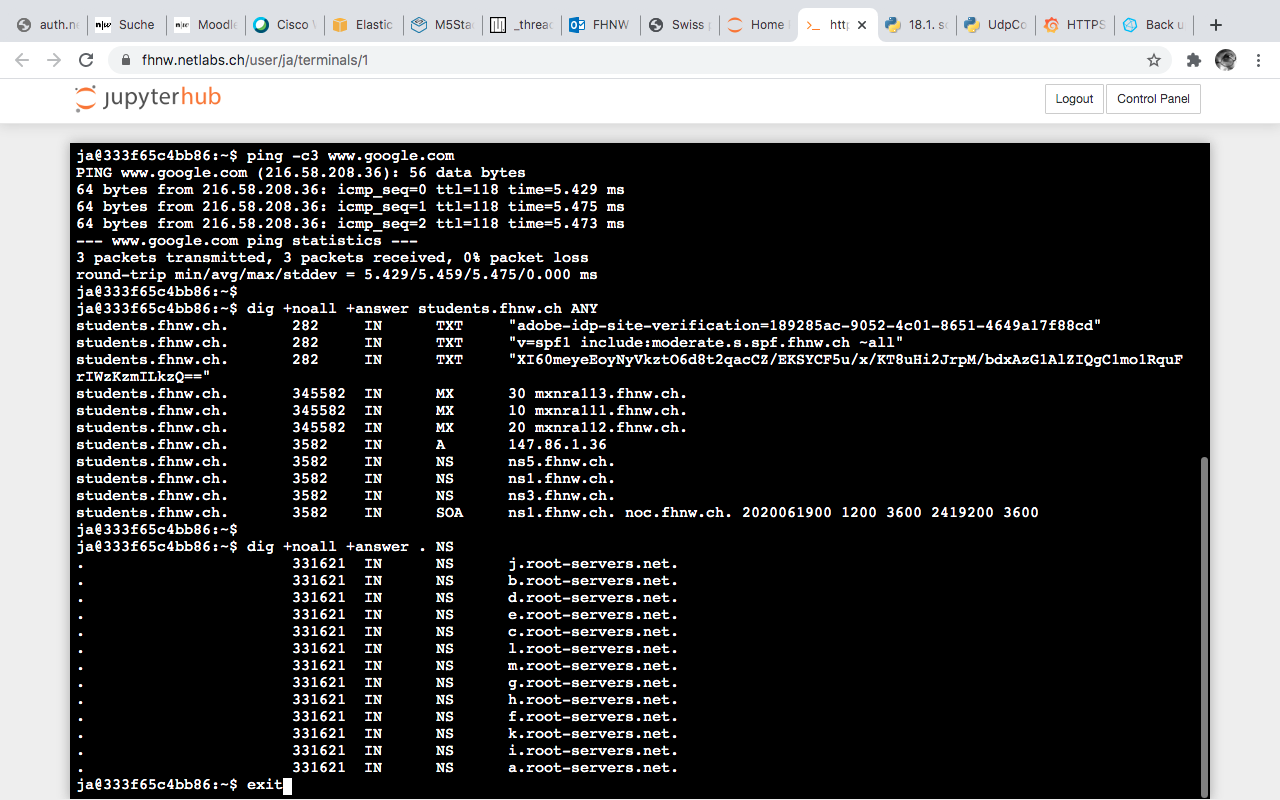
\includegraphics[width=10cm]{jupyterhub/jupyterhub_terminal}

\subsection*{Terminal verlassen}
Sie k\"onnen theroretisch einfach das Terminal-Fenster/Tab schliessen und/oder ``Logout'' aus dem Jupyternotebook das System verlassen -- das Terminal wird ``weiterlaufen'' (unter ``running'' im Jupyternotebook ersichtlich). 

Das Terminal bietet eine ``History'': Sie k\"onnen mit ``Pfeil aufw\"arts'' vorherige Kommandos wieder holen/editieren und erneut ausf\"uhren. Diese History bleibt auch erhalten, wenn Sie das Terminal stoppen.

Einen ``sauberen'' Stopp des Terminals wird mit dem Kommando \texttt{exit} erreicht (optional, sonst beim n\"achsten Login unter ``running'' das existieren Terminal wieder holen):

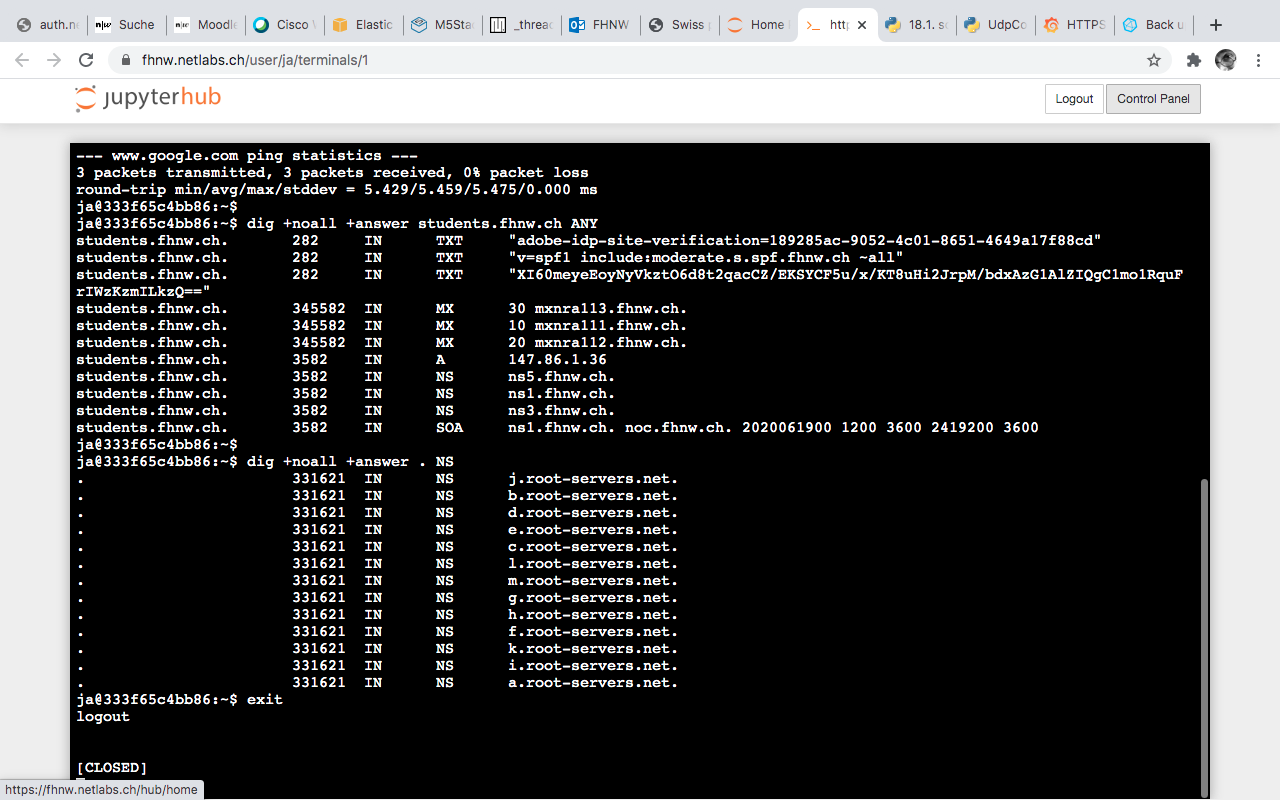
\includegraphics[width=10cm]{jupyterhub/jupyterhub_terminal_exit}


\subsection*{Terminal Ausgaben}
Terminal-Ausgaben k\"onnen sie einfach aus dem Fenster per Selektion kopieren. ``Advanced''-Benutzer k\"onnen auch mit ``$>$'' eine Ausgabe in eine Datei umleiten, die dann im Jupyternotebook erscheint: \texttt{dig +all +noshort . NS > root-servers.txt}

\end{document}